% To create a new appendix entry, add a new chapter and label to reference it 

\appendix
\appendixpage

\chapter{Test}
\label{appendix:test}

\chapter{Dependencies}
\label{appendix:dependencies}
\section{NPM dependencies}
\begin{itemize}
    \item @emotion/react@11.10.6
    \item @emotion/styled@11.10.6
    \item @microsoft/eslint-formatter-sarif@2.1.7
    \item @mui/material@5.11.13
    \item @playwright/test@1.31.2
    \item @testing-library/jest-dom@5.16.5
    \item @testing-library/react@13.4.0
    \item @testing-library/user-event@13.5.0
    \item @types/jest@27.5.2
    \item @types/node@16.18.16 
    \item @types/react-dom@18.0.11
    \item @types/react@18.0.28
    \item @typescript-eslint/eslint-plugin@5.56.0
    \item @typescript-eslint/parser@5.56.0
    \item axios@1.3.4
    \item eslint-plugin-react@7.32.2
    \item eslint@8.10.0
    \item mongodb@5.1.0
    \item playwright@1.31.2
    \item react-dom@18.2.0
    \item react-router-dom@6.9.0
    \item react-scripts@5.0.1
    \item react@18.2.0
    \item ts-md5@1.3.1
    \item typescript@4.9.5
    \item web-vitals@2.1.4
\end{itemize} 

\subsubsection{Dependency graph of npm package}
Example of a dependency graph for the npm package @playwright/test made from: \url{http://npm.anvaka.com/\#/view/2d/}

\begin{figure}[H]
    \centering
    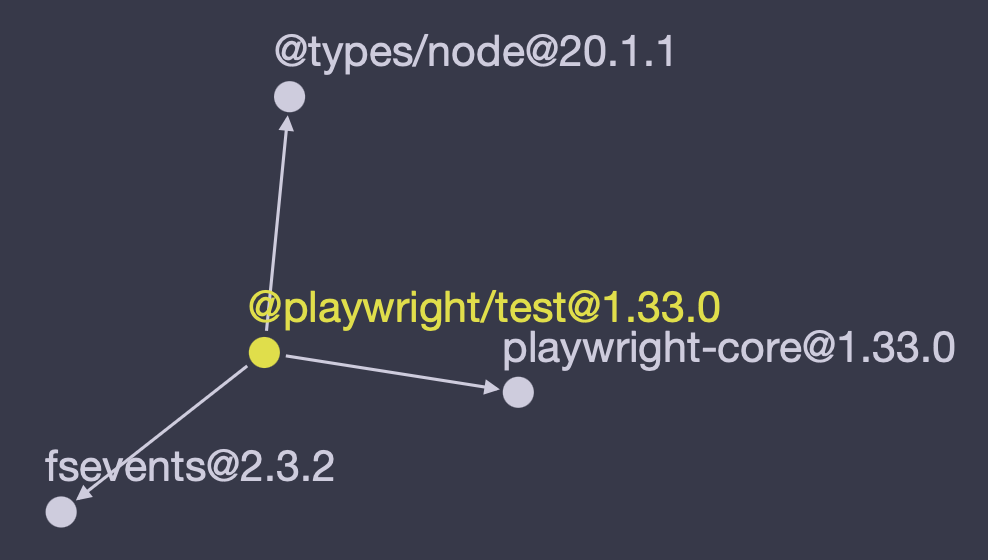
\includegraphics[width=10cm]{Report/img/playwrightDependency.png}
    \caption{Playwright dependency graph}
    \label{fig:playwrightDependencies}
\end{figure}


\subsection{C\# application dependencies}

\textit{MiniTwit.Core}
\begin{itemize}
    \item mapster
    \item Microsoft.AspNetCore.Mvc
    \item MongoDB.Bson
    \item MongoDB.Driver
\end{itemize}


\textit{MiniTwit.Infrastructure}
\begin{itemize}
    \item MongoDB.Driver
\end{itemize}

\textit{MiniTwit.Security}
\begin{itemize}
    \item Konscious.Security.Cryptography.Argon2
    \item Microsoft.Extensions.Options
\end{itemize}

\textit{MiniTwit.Server}
\begin{itemize}
    \item prometheus-net.AspNetCore  
    \item Serilog.AspNetCore    
    \item Serilog.Sinks.Grafana.Loki   
    \item Swashbuckle.AspNetCore 
\end{itemize}


\textit{MiniTwit.Tests/Infrastructure.Tests}
\begin{itemize}
   \item coverlet.collector 
   \item FluentAssertions  
   \item Microsoft.Extensions.Options   
   \item Microsoft.NET.Test.Sdk  
   \item Mongo2Go   
   \item Moq    
   \item xunit     
   \item xunit.runner.visualstudio  
\end{itemize}

\textit{MiniTwit.Tests/Server.Integration.Tests}
\begin{itemize}
   \item coverlet.collector 
   \item FluentAssertions  
   \item Microsoft.AspNetCore.Mvc.Testing    
   \item Microsoft.NET.Test.Sdk  
   \item Mongo2Go   
   \item xunit     
   \item xunit.runner.visualstudio  
\end{itemize}

\textit{MiniTwit.Tests/Server.Tests} 
\begin{itemize}
   \item coverlet.collector 
   \item Microsoft.AspNetCore.Mvc    
   \item Microsoft.NET.Test.Sdk  
   \item Moq   
   \item xunit     
   \item xunit.runner.visualstudio  
\end{itemize}










